\documentclass[tikz,border=10pt]{standalone}
\usepackage{amsmath,amssymb}
\usepackage{tikz}
\usetikzlibrary{arrows,automata,backgrounds,calendar,chains,decorations,decorations.pathreplacing,decorations.text,fit,matrix,mindmap,patterns,petri,plotmarks,positioning,shadows,shapes,shapes.callouts,shapes.geometric,shapes.misc,spy,trees,calc,intersections,tikzmark,arrows.meta}
\usepackage{xcolor}
\usepackage{pgfplots}
\pgfplotsset{compat=1.16}

% Common math macros from the book
\def\x{\mathbf{x}}
\def\y{\mathbf{y}}
\def\z{\mathbf{z}}
\def\A{\mathbf{A}}
\def\b{\mathbf{b}}
\def\c{\mathbf{c}}
\def\w{\mathbf{w}}
\def\v{\mathbf{v}}
\def\u{\mathbf{u}}
\def\e{\mathbf{e}}
\def\zero{\mathbf{0}}
\def\R{\mathbb{R}}
\def\N{\mathbb{N}}
\def\Z{\mathbb{Z}}
\def\Q{\mathbb{Q}}
\def\st{\text{s.t.}}
\def\vect#1{\mathbf{#1}}
\def\xLP{x^{\mathrm{LP}}}
\def\zLP{z^{\mathrm{LP}}}
\def\xIP{x^{\mathrm{IP}}}

% Common node styles from the book
\tikzset{
    main/.style={circle, draw, fill=gray!20, minimum size=1cm, font=\normalsize},
    dot/.style={circle,fill=blue,minimum size=3pt,inner sep=0pt, outer sep=-1pt},
    vertex/.style={circle,fill=black!25,minimum size=20pt,inner sep=0pt},
    edge/.style={draw,-,thick},
    directed edge/.style={draw,->,>=latex,thick},
}

% Additional macros for 3D/coordinate systems
\newcommand{\xhat}{\hat{\x}}
\newcommand{\yhat}{\hat{\y}}
\newcommand{\zhat}{\hat{\z}}
\newcommand{\ihat}{\hat{\imath}}
\newcommand{\jhat}{\hat{\jmath}}
\newcommand{\khat}{\hat{k}}

\begin{document}
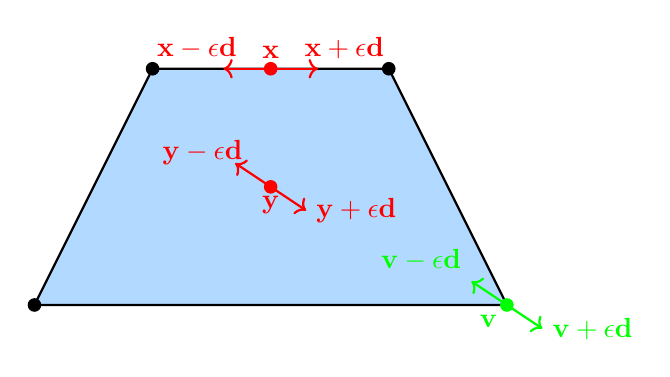
\begin{tikzpicture}[scale=1.5]
    % Draw the polytope
    \fill[blue!50!cyan,opacity=0.3] (0,0) -- (1,2) -- (3,2) -- (4,0) -- cycle;

    % Draw the edges of the polytope
    \draw[thick] (0,0) -- (1,2) -- (3,2) -- (4,0) -- cycle;

    % Label vertices
    \filldraw[black] (0,0) circle (1.5pt);
    \filldraw[black] (1,2) circle (1.5pt);
    \filldraw[black] (3,2) circle (1.5pt);
    \filldraw[green] (4,0) circle (1.5pt) node[below left] {$\mathbf{v}$};

    % Mark the point x on the edge
    \filldraw[red] (2,2) circle (1.5pt) node[above] {$\mathbf{x}$};

    % Draw the perturbation directions on the edge
    \draw[->, thick, red] (2,2) -- (2.4,2) node[midway, above right] {$\mathbf{x} + \epsilon \mathbf{d}$};
    \draw[->, thick, red] (2,2) -- (1.6,2) node[midway, above left] {$\mathbf{x} - \epsilon \mathbf{d}$};

    % Mark another point inside the polytope
    \filldraw[red] (2,1) circle (1.5pt) node[below] {$\mathbf{y}$};

    % Draw the perturbation directions inside the polytope
    \draw[->, thick, red] (2,1) -- (2.3,0.8) node[right] {$\mathbf{y} + \epsilon \mathbf{d}$};
    \draw[->, thick, red] (2,1) -- (1.7,1.2) node[midway, above left] {$\mathbf{y} - \epsilon \mathbf{d}$};

    % Draw perturbation directions for the green vertex
    \draw[->, thick, green] (4,0) -- (4.3,-0.2) node[right] {$\mathbf{v} + \epsilon \mathbf{d}$};
    \draw[->, thick, green] (4,0) -- (3.7,0.2) node[above left] {$\mathbf{v} - \epsilon \mathbf{d}$};

\end{tikzpicture}
\end{document}
